%%%%%%%%%%%%%%%%%%%%%%%%%%%%%%%%%%%%%%%%%
% Journal Article
% LaTeX Template
% Version 1.4 (15/5/16)
%
% This template has been downloaded from:
% http://www.LaTeXTemplates.com
%
% Original author:
% Frits Wenneker (http://www.howtotex.com) with extensive modifications by
% Vel (vel@LaTeXTemplates.com)
%
% License:
% CC BY-NC-SA 3.0 (http://creativecommons.org/licenses/by-nc-sa/3.0/)
%
%%%%%%%%%%%%%%%%%%%%%%%%%%%%%%%%%%%%%%%%%

%----------------------------------------------------------------------------------------
%	PACKAGES AND OTHER DOCUMENT CONFIGURATIONS
%----------------------------------------------------------------------------------------

\documentclass[twoside,twocolumn]{article}

\usepackage{blindtext} % Package to generate dummy text throughout this template 

\usepackage[sc]{mathpazo} % Use the Palatino font
\usepackage[T1]{fontenc} % Use 8-bit encoding that has 256 glyphs
\linespread{1.05} % Line spacing - Palatino needs more space between lines
\usepackage{microtype} % Slightly tweak font spacing for aesthetics

\usepackage[english]{babel} % Language hyphenation and typographical rules

\usepackage[hmarginratio=1:1,top=32mm,columnsep=20pt]{geometry} % Document margins
\usepackage[hang, small,labelfont=bf,up,textfont=it,up]{caption} % Custom captions under/above floats in tables or figures
\usepackage{booktabs} % Horizontal rules in tables

\usepackage{lettrine} % The lettrine is the first enlarged letter at the beginning of the text

\usepackage{enumitem} % Customized lists
\setlist[itemize]{noitemsep} % Make itemize lists more compact

\usepackage{abstract} % Allows abstract customization
\renewcommand{\abstractnamefont}{\normalfont\bfseries} % Set the "Abstract" text to bold
\renewcommand{\abstracttextfont}{\normalfont\small\itshape} % Set the abstract itself to small italic text

\usepackage{titlesec} % Allows customization of titles
\renewcommand\thesection{\Roman{section}} % Roman numerals for the sections
\renewcommand\thesubsection{\roman{subsection}} % roman numerals for subsections
\titleformat{\section}[block]{\large\scshape\centering}{\thesection.}{1em}{} % Change the look of the section titles
\titleformat{\subsection}[block]{\large}{\thesubsection.}{1em}{} % Change the look of the section titles

\usepackage{fancyhdr} % Headers and footers
\pagestyle{fancy} % All pages have headers and footers
\fancyhead{} % Blank out the default header
\fancyfoot{} % Blank out the default footer
\fancyhead[C]{System Design $\bullet$ Nov 2018} % Custom header text
\fancyfoot[RO,LE]{\thepage} % Custom footer text

\usepackage{titling} % Customizing the title section

\usepackage{hyperref} % For hyperlinks in the PDF

\usepackage{booktabs}
\usepackage{multirow}
\usepackage{framed}
\usepackage{caption}
\usepackage{graphicx}

%----------------------------------------------------------------------------------------
%	TITLE SECTION
%----------------------------------------------------------------------------------------

\setlength{\droptitle}{-4\baselineskip} % Move the title up

\pretitle{\begin{center}\Huge\bfseries} % Article title formatting
\posttitle{\end{center}} % Article title closing formatting
\title{System design report: Multi-Agent System} % Article title
\author{%
\textsc{James King} \\% Your name
\normalsize Supervisor: Kostas Stathis \\ % Your supervisor
}
\date{October 2018} % Leave empty to omit a date
\renewcommand{\maketitlehookd}{%
\begin{abstract}
\noindent Prolog services, Flask web application\\
https://users.ece.cmu.edu/~koopman/essays/abstract.html
\end{abstract}
}

%----------------------------------------------------------------------------------------

\begin{document}

%Milestone: Report on the design of the Prolog service and Agents, and the web application and agent’s environment
%Will include the following: an agent definition and the inner workings of an agent’s decision-making component, a definition of the structure of the Prolog service and management of agents (as well as the design of the API), a definition of the agent’s environment and how this will work with the Prolog service, and a design of the web application. This is key to a well-planned architecture for the Prolog service and agent environment. It will also help me research better methods of implementation for the Prolog service.
% Link to goal: This will lay out a concrete way of implementing the Prolog service, web application and link between them.

% Print the title
\maketitle

%----------------------------------------------------------------------------------------
%	ARTICLE CONTENTS
%----------------------------------------------------------------------------------------

\section{Introduction}
One of the aims of my project is to produce a multi-agent system to play games of indirect reciprocity, the model for which I have defined in my second report: ``Report on indirect reciprocity, strategies for agents and the development of a concrete model to implement''. For this I have designed a system that includes two main components: The environment and a web service to host agent's decision making components.\\
In my project I will be hosting the environment in my Flask web application, but, the aim is that the environment can be used as if it is a library as long as it is connected to an application/service that runs agent's decision making component. As such I will not be addressing how the web application hosting the environment, but the environment itself and the agents service.

%------------------------------------------------

\section{Content and Knowledge}
Talk about overall system design\\
Talk about choice between kostas' idea and mine.\\
Talk about proof of concept applications and lessons learnt from them.\\
Talk about learning from Annie Ogborne.\\
Talk about security: Prolog injection attacks, shell injection attacks, sql injection, remove library(http/http\_errors.pl) in production to make it harder
\subsection{Agents}
There are many different definitions of what properties a system needs in order to be considered an agent. One definition containing 4 properties was proposed by Wooldridge and Jennings~\cite{wooldridge_jennings_1995}: autonomy, reactivity, proactivity and social ability.\\
Autonomy being considered the ability to operate without direct human intervention and having control over the agent's own actions and internal state. Reactivity is defined as agents perceiving their environment and responding to changes in it in a timely fashion. Proactivity is given as the ability to exhibit goal-driven behaviour, rather than just reacting to it's environment. Lastly social ability is interaction between agents and/or humans via an ACL (agent communication language).\\
This `weak' notion of agency is widely accepted, but Wooldrige and Jennings note that some argue for a stronger notion that include human-like concepts. They have ppreviously mentioned one such notion: goals.\\
The goals of agents in game-theoretic models vary, two examples of goals are: maximising social welfare, help induce the evolution of cooperation and maximising your own fitness. The first example is attempted by the strategy always cooperate as always cooperating produces the maximum social welfare when using the payoff matrix in table~\ref{tab:payoffmatrix}.\\
\begin{framed}
	\begin{center}
		\begin{tabular}{c|c|c}
		\multirow{2}{*}{Donor Action} & \multicolumn{2}{c}{Payoffs}\\		
		& Donor & Recipient\\
		\hline
		Cooperation & -1 & 2\\
		\hline
		Defection & 0 & 0\\
		\end{tabular}
		\captionof{table}{The payoff used in my indirect reciprocity model}
		\label{tab:payoffmatrix}
	\end{center}	
\end{framed}
\noindent Due to the nature of the payoff matrix and the model, the last goal is not simple to reach. This is typical of many game-theoretic models, where generally strategies attempt to achieve it (with varying degrees of success) by encoding a theory of what is best to do when.\\
An example of this is the image scoring discriminator strategy as laid out by Nowak and Sigmud~\cite{evol_indirect_image}. This strategy encodes a theory that when interacting with another agent if the other agent's image score as perceived by the discriminator is greater than or equal to $k$ (a variable set at the initialization of the agent) it is best to cooperate, else the agent will defect.\\
Some strategies don't even have a goal and just seek to provide a theory to act on. Though this does not qualify them as an agent according to Wooldridge and Jennings~\cite{wooldridge_jennings_1995} they are still relevant strategies for game-theory.\\
These indirect reciprocity strategies have remarkable resemblance to how theories are encoded in deductive reasoning agents. Deductive reasoning agents use theories to encode how it is best to act under any given situation~\cite{kostas_deductive}. Agents who follow the image score discriminator strategy could have a theory encoded in them such as:
\begin{framed}
\noindent$interaction(me, Recipient, time) \wedge image\_score(me, Recipient, Score, time) \wedge Score\geq k \to do(cooperate(Recipient))$\\\\
$interaction(me, Recipient, time) \wedge image\_score(me, Recipient, Score, time) \wedge Score<k \to do(defect(Recipient))$\\\\
$\neg interaction(me, \_, time) \to do(idle)$
\end{framed}
\noindent Part of the deductive reasoning agents method of implementing agents is the logical database that includes information on the current state of the world. In the example above this would possibly include logical data such as:
\begin{framed}
\begin{center}
$image\_score(agent1, agent2, 2, 9).$ \\
$interaction(agent1, agent2, 6).$
\end{center}
\end{framed}
\noindent This logical database is similar to the human-like concept of belief that is included in the language Agent0 presented by Yoav Shoham~\cite{shoham1991agent0} as one of his two mental categories: belief and commitment.\\
He defines beliefs as a fact that is thought to be true by an agent at a specific time about a specific time (an agent is constrained to not believe contradictory facts). Commitments are given as a commitment to act (restricted by the agent's capabilities) not a commitment to pursue a goal.\\
Agent capabilities are another concept Shoham uses and are defined as relations between the agent's mental state and their environment. An agent is only capable of committing to an action iff they believe themself to be. In my example above this is shown by the agent only being capable of defecting or cooperating if they are a donor in an interaction.\\
In my system I wish to incorporate the idea of beliefs, commitments, capabilities and strategies (the theories encoded for an agent to decide how to act). Russell and Norvig specify that an agent can be thought of as a system perceives its environment and acts within it~\cite{russell2016artificial}. They then go on to explain that an agent maps percept sequences to actions. In the system I am producing this mapping will be provided by forming beliefs based on the percepts an agent receives and then deciding on an action to take based on these beliefs by way of a deductive reasoning theory.\\
Percepts in my system will include: an observation of an action (either cooperating or defecting), an observation of a gossip action (either positive or negative) and perceiving that they are a member of a donor-recipient pair at a given timepoint (and which role they hold).\\
\begin{figure}
	\begin{center}
	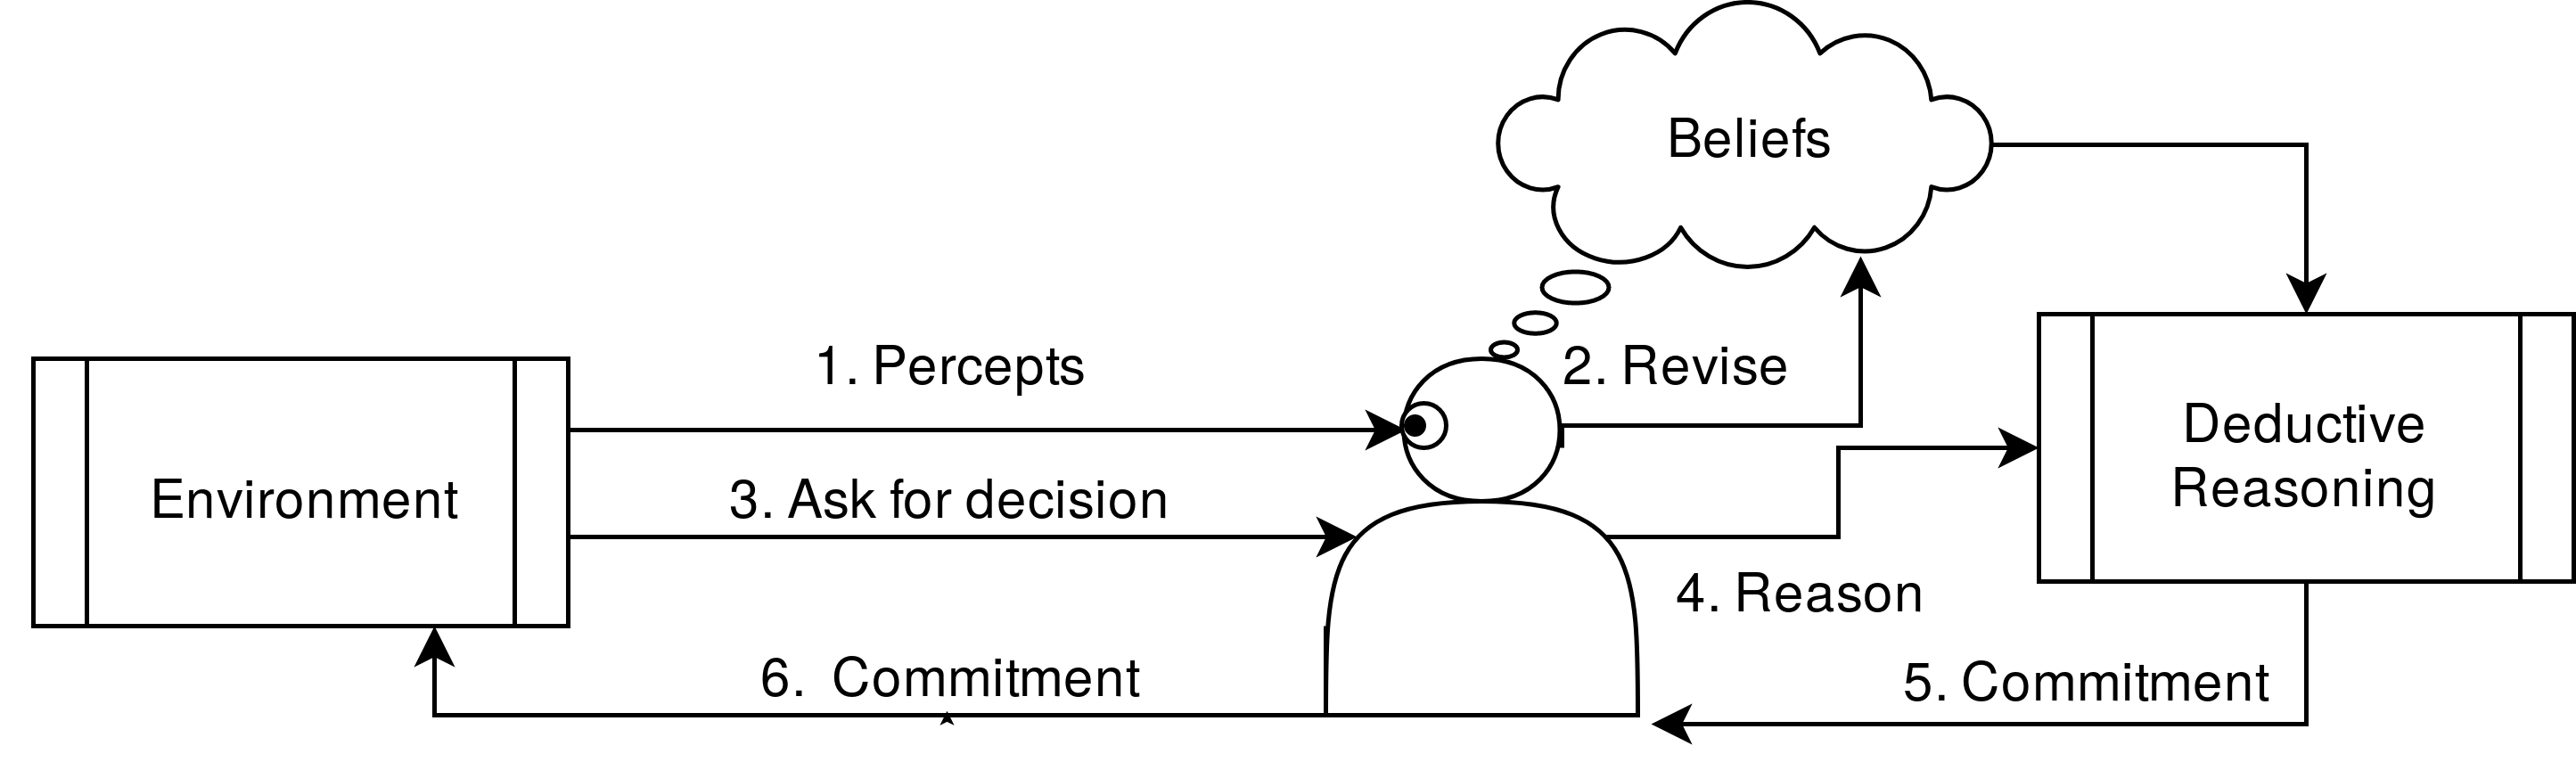
\includegraphics[width=0.5\textwidth]{PerceiveReviseDecide.png}
	\caption{Visual description of the process my agents' will follow}
	\label{fig:percept_to_action}
	\end{center}
\end{figure}
\noindent This raises the question: how do agents form beliefs based on the percepts they receive? The actual beliefs they will form based on percepts are strategy dependent, but the overriding concept is for the agents to follow a game-theoretic strategy.\\
To extend the example of the image scoring discriminator, let us say that agent1 perceives agent2 defecting against agent3. The image scoring strategy laid out by Nowak and Sigmund~\cite{evol_indirect_image} states that when a defection is perceived, the perceiving agent will lower the donor's image score in their beliefs.\\
Using this method percepts cause an agent's beliefs about it's environment and other agents to change at specific timepoints. This is remarkably similar to an approach to reasoning about events (similar to percepts) and time (timepoints) and how events change `fluents' (similar to beliefs) known as the event calculus, which was presented by Kowalski and Sergot~\cite{kowalski1989logic}.\\
Due to the remarkable similarities the use of the event calculus seems an intuitive way to program an agent to react to percepts and query beliefs. There is a version of the event calculus known as the multi-valued fluent cached event calculus (kindly provided by my supervisor) which will make querying beliefs efficient.\\
I have covered how agents will map from percepts to beliefs and then beliefs to actions. This will be executed in a cycle for each timepoint of an indirect reciprocity game, the cycles step includes in this order perceive, revise (works as a consequence of perceive) and decide. In the perceive step agents will receive percepts from the environment, passed through an API, from these percepts they will revise their beliefs. An agent will then decide on an action to take, the agent will commit to an action at the cycle step timepoint based on their beliefs. This matches a deductive reasoning style of agent and Russell and Norvig's definition of an agent~\cite{russell2016artificial}.\\
The capability of an agent will be constrained at a given timepoint by way of an agent perceiving that they are the donor of a donor-recipient pair at that timepoint. The decision on which agents are donors and recipients in pairs falls to the environment. If an agent perceives they are a donor they can only cooperate or defect, but when they are not they cannot cooperate or defect. At any other point when they are not a donor they will be able to gossip or be idle.\\
In conclusion I believe that the agent structure I have delineated matches the 4 properties Wooldridge and Jennings described~\cite{wooldridge_jennings_1995}. Autonomy has been satisfied by way that agents have control over their beliefs, control over the actions they commit to based on these beliefs and merely choose to act based on their environment not human action. Reactivity is satisfied by the process of receiving percepts, formulating beliefs from them, and then being able to respond to the changes in the environment by acting based on these beliefs.\\
In my system agents have 5 options as to the actions they will be able to take: idle, positive gossip, negative gossip, cooperate as a donor and defect as a donor. Both the last two properties are met by the possibility of gossip actions, and for proactivity the ability to choose between cooperating and defecting. Gossip actions are communicative actions where a gossiper communicates to another agent either positive or negative ideas about a third agent, displaying social ability. Gossip actions also show proactivity as agents can actively seek to inform other agents in a way that will affect the overall game to being them closer to their goal.\\
An example of this is an agent who's goal it is to induce the evolution of cooperation gossiping to another agent a negative idea about an agent that it has viewed defecting, in the hope that the recipient of the gossip will then not help the defector by cooperating with them if they're a donor.

\subsection{Environment}


\subsection{Communication and API Design}


%------------------------------------------------

\section{Discussion and Conclusion}
Secur


%----------------------------------------------------------------------------------------
%	REFERENCE LIST
%----------------------------------------------------------------------------------------

\bibliography{../refs.bib}{}
\bibliographystyle{plain}

%----------------------------------------------------------------------------------------

\end{document}
